\documentclass[12pt]{exam}
\usepackage[portuguese]{babel}
\usepackage[utf8]{inputenc}
\usepackage{graphicx}
\graphicspath{{figuras/}}

\usepackage[margin=1in]{geometry}
\usepackage{amsmath,amssymb}
\usepackage{multicol}
\usepackage{textcomp,lmodern,listings}
\lstset{language=SQL,basicstyle=\ttfamily, columns=fullflexible, upquote, morekeywords={data,wrapper,library,language}}

\newcommand{\disciplina}{Banco de Dados}
\newcommand{\class}{\disciplina}
\newcommand{\term}{Professor: Igor Avila Pereira}
\newcommand{\bimestre}{1}
\newcommand{\valor}{4}
\newcommand{\examnum}{Prova 2 - \bimestreº Bimestre - Valor: \valor}
%\newcommand{\examdate}{xx}
%\newcommand{\timelimit}{4 horas}

\pagestyle{head}
\firstpageheader{}{}{}
\runningheader{\class} - {Página \thepage\ de \numpages}
\runningheadrule


\begin{document}

\noindent
\begin{tabular*}{\textwidth}{l @{\extracolsep{\fill}} r @{\extracolsep{6pt}} l}
\textbf{\class} & \textbf{Nome:} & \makebox[2in]{\hrulefill}   \\
\textbf{\examnum} & \textbf{Matrícula:} & \makebox[2in]{\hrulefill}   \\
%\textbf{\examnum} &&\\
%\textbf{\examdate} &&\\
\textbf{\term} &&\\
%\textbf{Duração: \timelimit}
\end{tabular*}\\
\rule[2ex]{\textwidth}{2pt}
\noindent
%rule[2ex]{\textwidth}{2pt}

\begin{questions}


\question (1.0) Construa um DER para o gerenciamento de gravadoras de CD's onde:

\begin{itemize}
    \item Um \textbf{autor} tem \textbf{id} e um \textbf{nome} (texto não-nulo);
    \item Uma \textbf{música} tem \textbf{id}, \textbf{nome} (texto não-nulo) e \textbf{duração} (tempo);
    \item Uma \textbf{gravadora} tem \textbf{id}, \textbf{nome} (texto não-nulo), \textbf{endereço} (texto), \textbf{telefone} (texto), \textbf{contato} (texto) e \textbf{site} (texto)
    \item Um \textbf{CD} tem \textbf{id}, \textbf{nome}, \textbf{preço} (número real não-nulo e $> 0$), \textbf{data de lançamento} (data com valor padrão sendo a data atual)
    \item Além disso:
    \begin{itemize}
        \item Um \textbf{autor pode compor várias músicas e uma música pode ser composta por vários autores};
    \item \textbf{Um música pode estar em vários CD's e um CD pode ter várias músicas (faixas)}. Além disso, deve-se armazenar o \textbf{número da faixa} que cada música teve nos CD's que participou/integrou;
        \item Músicas podem não ter nenhum autor;
        \item \textbf{Uma gravadora produz vários CD's e um CD é produzido, exclusivamente, por uma única gravadora};
        \item \textbf{Para cada CD cadastrado na base dados é possível indicar um outro CD da base de dados, ou seja, cada CD pode recomendar um outro CD e, assim, sucessivamente};
    \end{itemize}
\end{itemize}
\begin{itemize}
    \item \textbf{Dica:} Use o DIA e cuidado com as cardinalidades n:n.
\end{itemize}

% \textbf{Gabarito:}
% \begin{figure}[!htp]
% \centering
% 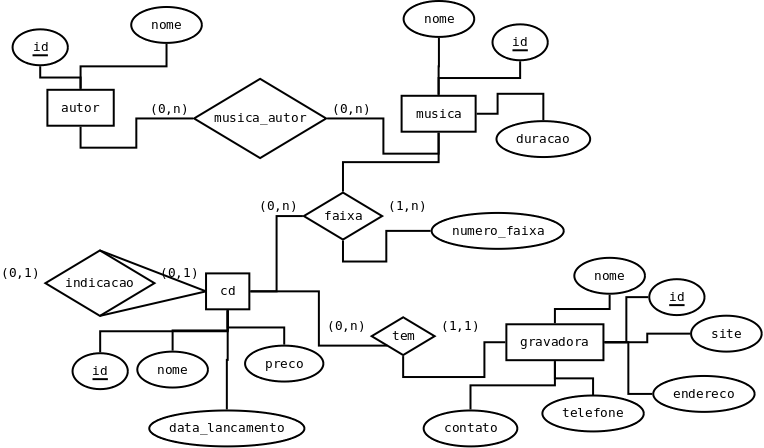
\includegraphics[width=0.7\linewidth]{figuras/prova-er.png}
% \end{figure}

% \newpage

\question (1.0) Construa o modelo relacional do exercício anterior.

\begin{itemize}
    \item \textbf{Dica:} Use o DIA, cuidado com as chaves primárias compostas e as tabelas intermediárias resultantes de relacionamentos n:n.
\end{itemize}

% \begin{figure}[!htp]
% \centering
% 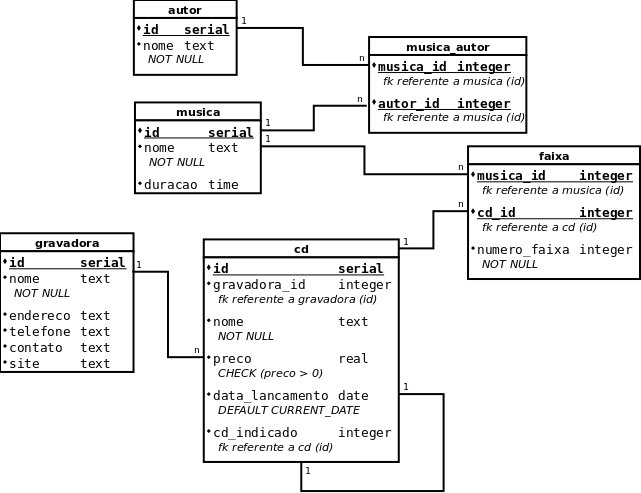
\includegraphics[width=0.9\linewidth]{figuras/prova-modelo-relacional.png}
% %\caption{Questão \ref{fig:funcionarios_dependentes}}
% % \label{fig:funcionarios_dependentes}
% \end{figure}

\question (0.5) Construa o \textit{script.sql} de criação do B.D do modelo relacional desenvolvido no exercício anterior 
\begin{itemize}
    \item \textbf{Dica:} CREATE DATABASE, CREATE TABLE, PRIMARY KEY, FOREIGN KEY, CHECK, NOT NULL e etc.
\end{itemize}

% \textbf{Gabarito:}
% \begin{verbatim}
% DROP DATABASE IF EXISTS gravadora;
% CREATE DATABASE gravadora;
% \c gravadora;
% CREATE TABLE autor (
%     id serial primary key,
%     nome text not null
% );
% CREATE TABLE musica (
%     id serial primary key,
%     nome text not null,
%     duracao time
% );
% CREATE TABLE musica_autor (
%     musica_id integer references musica (id),
%     autor_id integer references autor (id),
%     primary key (musica_id, autor_id)
% );
% CREATE TABLE gravadora (
%     id serial primary key,
%     nome text not null,
%     endereco text,
%     telefone text,
%     contato text,
%     site text
% );
% CREATE TABLE cd (
%     id serial primary key,
%     gravadora_id integer references gravadora (id),
%     nome text not null,
%     preco real not null check (preco > 0),
%     data_lancamento date DEFAULT CURRENT_DATE
% );
% CREATE TABLE faixa (
%     musica_id integer references musica (id),
%     cd_id integer references cd (id),
%     numero_faixa integer not null,
%     primary key (musica_id, cd_id)
% );
% \end{verbatim}

\question (0.5) Além das instruções necessárias para criação do B.D, construa instruções SQL necessárias para \textbf{\underline{INSERIR}} no B.D os seguintes dados:

\begin{itemize}
    \item \textbf{4 gravadoras}
    \item \textbf{4 autores}
    \begin{itemize}
        \item Destes autores:
        \begin{itemize}
            \item Pelo menos 1 com nome começando com R e terminando com O. 
            \begin{itemize}
                \item Ex: Renato Russo
            \end{itemize}
        \end{itemize}
    \end{itemize}
    \item \textbf{4 cd's}
    \begin{itemize}
        \item Destes cd's:
        \begin{itemize}
            \item Pelo menos 2 cd's com datas de lançamento $\geq 1995$ e $\leq 2000$
            % \item Insira com nome, preço e data de lançamento
        \end{itemize}
         \item \textbf{Dica:} Estas instruções SQL devem atribuir nome, preço, data de lançamento e alguma gravadora para estes cd's.
    \end{itemize}
    \item \textbf{4 músicas}
        \begin{itemize}
            \item Destas músicas:
            \begin{itemize}
                \item Uma ou mais músicas \textbf{devem ter mais de um autor};
                \item Uma ou mais músicas devem \textbf{não ter autor};
                \item \textbf{Pelo menos 2 músicas devem ter sido composta por um mesmo autor}, ou em outras palavras, \textbf{um mesmo autor tem ser autor de mais de uma música cadastrada};
            \end{itemize}
            \item \textbf{Dica:} Nas músicas com autor(es) é preciso criar também instruções SQL de inserção para tabelas intermediárias que possam surgir durante o mapeamento do DER para o Modelo Relacional (Ex: tabela \textbf{musica\underline{\hspace{0.3cm}}autor})
        \end{itemize}
\end{itemize}

% \textbf{Gabarito:}
% \begin{verbatim}
% INSERT INTO gravadora (nome) VALUES 
% ('Universal'),
% ('Trama'),
% ('Sony'),
% ('Poligram');

% INSERT INTO autor (nome) VALUES 
% ('Peninha'),
% ('Renato Russo'),
% ('Michael Sullivan'),
% ('Massadas'),
% ('José Augusto');

% INSERT INTO musica (nome) VALUES 
% ('Alma Gemea'),
% ('País e Filhos'),
% ('Tarde De Domingo'),
% ('Que país é esse?'),
% ('Envolver');

% INSERT INTO musica_autor (musica_id, autor_id) VALUES 
% (1,1),
% (2,2),
% (3,3),
% (4,2),
% (2,4);

% INSERT INTO cd (nome, preco, data_lancamento, gravadora_id) VALUES 
% ('Legião Urbana - CD', 10.0, '1990-05-05', 1),
% ('Tim maia', 23.0, '1995-04-06', 2),
% ('Fabio Jr.', 12.0, '2000-11-10', 1),
% ('Rita Lee.', 10.0, '2000-11-10', 1);
% \end{verbatim}

% \newpage

% \question (0.1) Construa a instrução SQL para \textbf{\underline{ATUALIZAR}} o \textbf{nome} de uma gravadora por seu id específico.
% \textbf{Gabarito:}
% \begin{verbatim}
%  UPDATE gravadora SET nome = 'Novo Nome da Gravadora' WHERE id = ?;
% \end{verbatim}

% \question (0.1) Construa a instrução SQL pra \textbf{\underline{DELETAR}} um cd específico pelo seu id.
% \textbf{Gabarito:}
% \begin{verbatim}
%  DELETE FROM cd WHERE id = ?;
% \end{verbatim}


% \question  Construa a instrução SQL que selecione o nome da gravadora e o nome dos CDs onde o id da gravadora seja 2 ou 3.
% \textbf{Gabarito:}
% \begin{verbatim}
%  SELECT gravadora.nome, cd.nome FROM gravadora 
% INNER JOIN cd ON (gravadora.id = cd.gravadora_id) 
% WHERE gravadora.id = 2 or gravadora.id = 3;
% \end{verbatim}


\question (0.2)  Construa a instrução SQL que mostre os \textbf{nome} dos \textbf{autores} que tem o \textbf{nome} \textbf{começando com R e terminando com O}. Ex: Renato Russo, Roberto Gusmão e etc.

\begin{itemize}
    \item \textbf{Dica:} Funções de Manipulação de \textit{Strings}
\end{itemize}

% \textbf{Gabarito:}
% \begin{verbatim}
%  SELECT nome FROM autor WHERE nome ILIKE 'R%O';
% \end{verbatim}


% \question Construa a instrução SQL que mostre o nome da música e o nome do autor ordenados pelo id da música.
% \begin{verbatim}
%  SELECT musica.nome, autor.nome FROM autor 
% INNER JOIN musica_autor ON (autor.id = musica_autor.autor_id) 
% INNER JOIN musica ON (musica.id = musica_autor.musica_id) 
% ORDER BY musica.id;
% \end{verbatim}

% \question  Mostre o nome dos CD's de uma gravadora (baseado no seu id) ordenados por nome de cada CD.
% \begin{verbatim}
%  select cd.nome FROM gravadora INNER JOIN cd ON (gravadora.id = cd.gravadora_id) 
% WHERE gravadora.id = 1 ORDER BY cd.nome;
% \end{verbatim}

% \question Liste o nome das músicas e seus correspondentes autores.
% \begin{verbatim}
%  SELECT autor.nome, musica.nome FROM autor 
% INNER JOIN musica_autor ON (autor.id = musica_autor.autor_id) 
% INNER JOIN musica ON (musica.id = musica_autor.musica_id) 
% ORDER BY musica.nome;
% \end{verbatim}

% \question Construa a instrução SQL que conte quantas músicas não possuem autores.
% \begin{verbatim}
%  SELECT count(*) FROM musica 
% WHERE id NOT IN (SELECT musica_id FROM musica_autor);
% \end{verbatim}


\question (0.2)  Construa a instrução SQL que mostre somente as músicas que \textbf{NÃO} tem autores.

\begin{itemize}
    \item \textbf{Dica:} SUBSELECT ou EXCEPT
\end{itemize}

% \textbf{Gabarito:}
% \begin{verbatim}
% SELECT musica.nome FROM musica 
% WHERE id NOT IN (SELECT musica_id FROM musica_autor);
% \end{verbatim}

% \question Mostre os autores que não tem nenhum música cadastrada.
% \begin{verbatim}
%  SELECT nome FROM autor 
% WHERE id NOT IN (SELECT autor_id FROM musica_autor);
% \end{verbatim}

\question (0.2)  Construa a instrução SQL que mostre o \textbf{nome} do CD e a \textbf{data de lançamento} dos CD's que foram lançados entre os anos de 1995 (inclusive) e 2000 (inclusive)

\begin{itemize}
    \item \textbf{Dica:} EXTRACT
\end{itemize}

% \textbf{Gabarito:}
% \begin{verbatim}
% SELECT nome, data_lancamento FROM cd 
% WHERE extract(year from data_lancamento) >= 1995 
% AND extract(year from data_lancamento) <= 2000;
% \end{verbatim}


% \question  Construa a instrução SQL que mostre a \textbf{quantidade} de músicas compostas por cada autor. Obs: mostrar também o \textbf{nome} dos autores.
% \begin{verbatim}
%  select autor.nome, count(*) from autor 
% INNER JOIN musica_autor ON (autor.id = musica_autor.autor_id) 
% INNER JOIN musica ON (musica.id = musica_autor.musica_id) 
% GROUP BY autor.nome;
% \end{verbatim}

\question (0.2) Construa a instrução SQL que mostre para cada gravadora: o \textbf{nome}, o \textbf{preço médio} de seus CDs, o \textbf{maior preço} entre seus cd's, o \textbf{menor preço} entre seus cd's e \textbf{a quantidade} de CDs.

\begin{itemize}
    \item \textbf{Dica:} Funções de agregação, Junção de Tabelas e GROUP BY
\end{itemize}

% \textbf{Gabarito:}
% \begin{verbatim}
% SELECT gravadora.nome, avg(cd.preco), 
% max(cd.preco), min(cd.preco), count(*) FROM gravadora 
% INNER JOIN cd ON (gravadora.id = cd.gravadora_id)
% GROUP BY gravadora.nome;
% \end{verbatim}

\question (0.2) Construa a instrução SQL que selecione o \textbf{nome} das músicas e a \textbf{quantidade de autores} das músicas que tem mais de um autor, ou seja, quantidade de autores $\geq 2$

\begin{itemize}
    \item \textbf{Dica:} Funções de agregação, Junção de Tabelas, GROUP BY e HAVING
\end{itemize}

% \textbf{Gabarito:}
% \begin{verbatim}
% SELECT musica.nome, count(*) FROM autor 
% INNER JOIN musica_autor ON (autor.id = musica_autor.autor_id) 
% INNER JOIN musica ON (musica.id = musica_autor.musica_id) 
% GROUP BY musica.nome HAVING count(*) >= 2;
% \end{verbatim}


\end{questions}
\end{document}